\section{Organizační struktura pevného disku operačním systémem Windows}
\subsection{Rozdělení disku na oblasti}
Disk je rozdělen do několika oblastí, známých jako partition nebo oddíly, aby bylo možné efektivně spravovat a organizovat data. Hlavní typy oddílů jsou primární, rozšířené a logické. Primární oddíly mohou obsahovat operační systém, zatímco rozšířený oddíl může obsahovat několik logických oddílů. Každý oddíl může být formátován s různými souborovými systémy, jako jsou NTFS, FAT32 nebo exFAT.

\subsection{MBR, EPT a GPT}
\paragraph{MBR}
Master Boot Record (MBR) je tradiční metoda pro rozdělení disku, která existuje od roku 1983. MBR obsahuje tabulku oddílů s maximálně čtyřmi záznamy, z nichž jeden může být rozšířený oddíl. Rozšířený oddíl lze dále dělit na logické disky pomoci tabulek rozšířených 
segmentů – EPT. MBR také obsahuje malý spustitelný kód, který pomáhá při zavádění operačního systému. MBR je omezen na disky o velikosti do 2 TB a podporuje maximálně čtyři primární oddíly.

\begin{figure}[h]
\centering
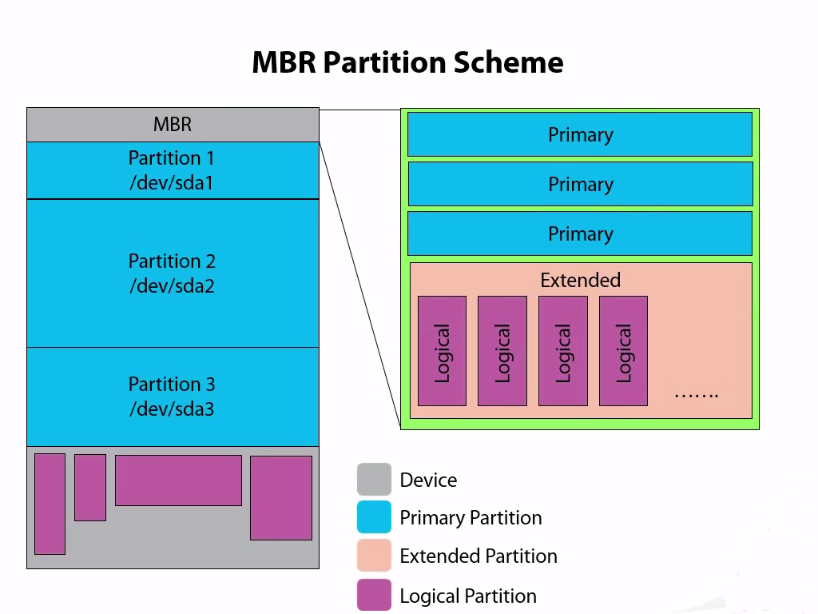
\includegraphics[scale=0.3]{sections/14_org_struk_pev_disk_op_sys_win/images/2-2128175945.png}
\end{figure}

\paragraph{GPT}
GUID Partition Table (GPT) je moderní metoda rozdělení disku, která je součástí standardu UEFI. GPT umožňuje vytvářet disky větší než 2 TB a podporuje až 128 oddílů na jednom disku (v systému Windows). GPT také poskytuje redundantní záhlaví a tabulky oddílů na začátku a na konci disku, což zvyšuje spolehlivost a integritu dat.

\begin{figure}[h]
\centering
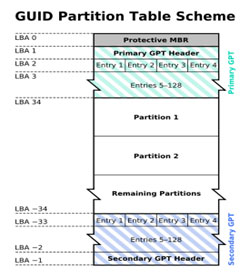
\includegraphics[scale=0.5]{sections/14_org_struk_pev_disk_op_sys_win/images/gpt-scheme-26093702.jpg}
\end{figure}

\subsection{PAT, EPT a program Diskedit}
\paragraph{PAT}
Partition Allocation Table (PAT) je datová struktura, která definuje, jak je disk rozdělen na jednotlivé oddíly.

\paragraph{EPT}
Extended Partition Table (EPT) V rozšířeném oddílu lze vytvořit více logických disků (každý logický disk má svoji EPT). Její funkce je ukázat na další EPT v rozšířené oblasti a propojit tak jednotlivá oddělení disku. Počet tabule EPT je tolik, kolik je logických disků uvnitř rozšířeného oddílu.

\paragraph{Program Diskedit}
Diskedit je nástroj pro přímou editaci sektorů disku, používaný často pro nízkoúrovňové úpravy a obnovu dat. Diskedit umožňuje zobrazit a upravit obsah diskových sektorů, což může být užitečné při obnově poškozených oddílů nebo při analýze struktury souborového systému.

\subsection{Programy pro správu disků Acronis Disk Director a Paragon Partition Manager}
Acronis Disk Director a Paragon Partition Manager jsou nástroje pro správu disků, které umožňují uživatelům vytvářet, mazat, rozdělovat, slučovat a upravovat oddíly na disku. Tyto programy poskytují uživatelsky přívětivé rozhraní a pokročilé funkce, jako je změna velikosti oddílů bez ztráty dat, zálohování a obnova oddílů, a klonování disků.

\subsection{Adresování CHS a LBA, souvislost s BIOSem a UEFI}
\paragraph{CHS}
Cylinder-Head-Sector (CHS) je starší metoda adresování sektorů na pevném disku, která používá tři čísla: cylindr, hlavu a sektor. CHS adresování je omezeno na disky s maximální kapacitou 8.4 GB a bylo nahrazeno metodou LBA kvůli své složitosti a omezením.

\paragraph{LBA}
Logical Block Addressing (LBA) je moderní metoda adresování sektorů, která používá sekvenční čísla pro každý sektor na disku, což zjednodušuje správu a umožňuje podporu větších disků. LBA je podporováno moderními BIOSy a UEFI.

\begin{figure}[h]
\centering
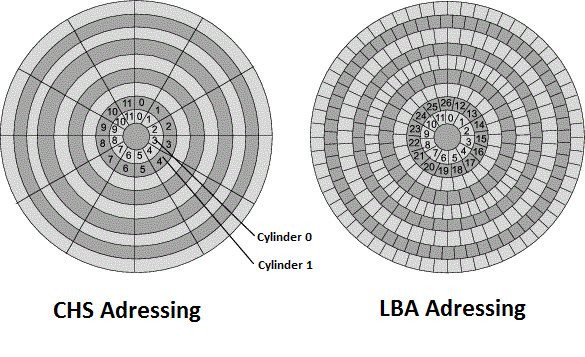
\includegraphics[scale=0.3]{sections/14_org_struk_pev_disk_op_sys_win/images/chs_lba-890647175.jpg}
\end{figure}


\subsection{EFI system partition, vznik, obsah}
EFI System Partition (ESP) je speciální oddíl na disku, který obsahuje soubory potřebné pro zavádění operačního systému v prostředí UEFI. ESP vzniká při instalaci operačního systému na disky formátované s GPT. Obsahuje bootovací zavaděče, ovladače a další soubory potřebné pro inicializaci systému. Typicky má velikost mezi 100 MB a 500 MB a je formátován s FAT32 souborovým systémem. ESP je klíčový pro správnou funkci UEFI a umožňuje snadné zavádění a správu různých operačních systémů na jednom disku.